\chapter{Detectors, Clocks, and Event Tables}
\label{chap:e13}

\begin{chapteropening}
Chapter~\ref{chap:e07} told us that the essence of detection is "absorb one photon, spit out one electrical pulse"; Chapter~\ref{chap:e08} then told us that the correlation peak hidden in the event stream can be as small as $10^{-6}$, and will be convolutionally broadened and diluted by the detector's finite temporal response. Yet both of those chapters still remained at the level of an "ideal detector." Real telescopes have no ideal detector: a photon striking the photocathode has only a certain probability of turning into an electron; the arrival time of each electrical pulse carries a random jitter of tens of picoseconds to a few nanoseconds; every time the detector fires it must "catch its breath," blind to new photons during this dead time; and the clocks of two telescopes a hundred metres apart must still be aligned to the picosecond. This chapter answers a very "hardware" question: a photon, through exactly which stages does it pass before it becomes that one \emph{time-stamped record} in the event table? We will take apart quantum efficiency, timing jitter, dead time and pile-up, afterpulsing, and clock synchronization one by one, deriving every formula from beginning to end, and finally landing on the most practical checklist of all: "which fields should the event table store?"
\end{chapteropening}

\section{From a photon to one time-stamped event}
\label{sec:e13-from-photon-to-event}

Let us first catch the conclusion of the previous stage. Chapter~\ref{chap:e07} described "detection" as a probabilistic event: a photon of energy $h\nu$ strikes the detector and has a certain probability of being absorbed and triggering a recordable electrical pulse. Chapter~\ref{chap:e08} lined up these electrical pulses into a string of time-stamped "clicks," and taught us to read $g^{(2)}(\tau)$ out of them. But the detector there was "transparent": photons in, events out, with no loss, delay, or saturation in between. Real devices are exactly the opposite: they set up several checkpoints between the photon and the event, and each checkpoint rewrites the event rate, the time stamp, or the peak shape. This chapter is about opening up each of these checkpoints one by one.

The key data structure is called the \textbf{event table} (event list). It differs fundamentally from an ordinary light curve. A light curve is "accumulate the photon count of a stretch of exposure into one time bin", once accumulated, who came at what moment, from which telescope, at which wavelength, in which polarization, is all smeared into a single number. The event table is the opposite: it preserves information \emph{photon by photon}: arrival time, telescope number, detector channel, wavelength channel, polarization channel, weight, quality flag. Why is it worth being this "verbose" in storage? Because for measurements such as second-order correlation, pulsar folding, and rapid occultation, the signal is hidden precisely in the joint information of "which two photons arrived almost simultaneously"; as soon as you accumulate into time bins too early, the correlation peak you seek is erased and can never be recovered afterwards. Iqueye was designed this way: it saves every photon with a time tag, then offline selects any time bin from 24.41 ps to minute scale; a single observation of $\zeta$ Ori produced about $2\times10^{10}$ photon events, about 78 GB of data \citep{2009A&A...508..531N,2019CoSka..49...85Z}. Clearly the event table is not an optional auxiliary file but the primary data product of a real telescope.

Writing down one raw event, it looks like this:
\begin{equation}
  \mathcal{E}^{\rm raw}_q =
  \big(n_q,\ a_q,\ d_q,\ c_q,\ p_q,\ f_q,\ w_q\big),
  \qquad
  t^{\rm raw}_q=t_0+n_q\,\delta t+\epsilon_{\rm roll}.
  \label{eq:e13-raw-event}
\end{equation}
\begin{formulaexplain}
$\mathcal E_q^{\rm raw}$ is the $q$-th raw event; $n_q$ is the clock count (tick), $\delta t$ is the duration of one tick, $t_0$ is the start of the recording segment, and $\epsilon_{\rm roll}$ handles counter overflow. It translates one electronic record into the earliest event time.
\end{formulaexplain}
Let us pin down each symbol. The subscript $q$ numbers the $q$-th event. $n_q$ is the integer number of ticks read by the electronic counter (dimensionless); $\delta t$ is the time corresponding to one tick (units of seconds), and for modern time-to-digital converters (TDCs) $\delta t$ is often in the range $10^{-11}$--$10^{-10}\,{\rm s}$; commercial multi-channel TCSPC systems can reach a basic timing resolution of 80 ps, and Iqueye's quantization step is 24.41 ps \citep{2009A&A...508..531N,2020RScI...91a3108W}. $t_0$ is the start moment of the recording segment (seconds), and $\epsilon_{\rm roll}$ handles counter rollover after reaching full scale, or segmentation. The remaining integers are all "labels": $a_q$ is the telescope or station number, $d_q$ is the detector number, $c_q$ is the wavelength channel or filter number, $p_q$ is the polarization channel, $f_q$ is the quality flag, and $w_q$ is the event weight. Overflows, dropped packets, saturation, clouds, pointing anomalies, and electronics anomalies should all be written into $f_q$; otherwise, when a strange peak later appears in the correlation function, you will have no way to trace whether it is celestial or a fault.

\begin{figure}[tbp]
\centering
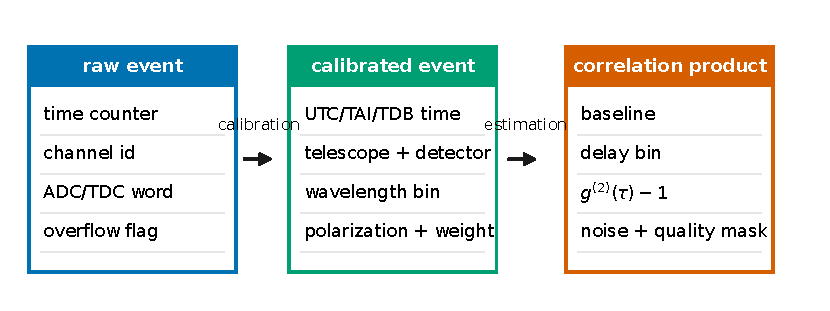
\includegraphics[width=0.96\linewidth]{figures/generated/chapter_06/ch06_event_table_schema.pdf}
\caption{Event data flow from the raw electronic record to the calibrated event table, and then to the correlation-function product. The raw layer stores counter time, channel numbers, and overflow flags; the calibrated layer converts time to a unified time scale and adds telescope, wavelength, polarization, and weight; the correlation-product layer finally records baseline, delay bin, correlation amplitude, and noise estimate. If only the light curve is stored at the first layer, the later clock, wavelength, and polarization selections can no longer be re-executed.}
\label{fig:e13-event-table-schema}
\end{figure}

The road map of this chapter is therefore clear: first look at how a photon turns into an electron event with probability $\eta$ (Section~\ref{sec:e13-detectors}), then look at how much jitter each event time carries and how it convolutionally widens the correlation peak (Section~\ref{sec:e13-jitter}), then look at how the "catching-breath" dead time and pile-up cause the recording rate to saturate (Section~\ref{sec:e13-deadtime}), how afterpulsing forges a short-delay correlation (Section~\ref{sec:e13-afterpulse}), then align the clocks of two telescopes to the picosecond (Section~\ref{sec:e13-clock}), and finally land on the event-table field checklist (Section~\ref{sec:e13-schema}) and the trade-off between spectral resolution and coherence time (Section~\ref{sec:e13-spectral}).

\section{Detectors: quantum efficiency turns photons into electron events}
\label{sec:e13-detectors}

The first and most basic role of a detector is to determine "how many incident photons really became electron events." The core parameter of this step is called the \textbf{quantum efficiency} $\eta$: the probability that a photon arriving at the photosensitive surface is absorbed and triggers one countable pulse. It is dimensionless, takes values between 0 and 1, and depends strongly on wavelength. Multiplying together the efficiencies along the entire optical path, the mean detection rate of a channel is
\begin{equation}
  R_{\rm det}
  =
  A_{\rm eff}
  \int_{\lambda_1}^{\lambda_2}
  F_\lambda(\lambda)\,
  T_{\rm opt}(\lambda)\,
  \eta(\lambda)\,
  d\lambda
  \;+\;R_{\rm sky}+R_{\rm dark}.
  \label{eq:e13-detected-rate}
\end{equation}
\begin{formulaexplain}
$R_{\rm det}$ is the detected count rate; $A_{\rm eff}$ is the effective collecting area; $F_\lambda$, $T_{\rm opt}$, $\eta$ are respectively the source photon spectral flux, the optical-path transmission, and the quantum efficiency; $R_{\rm sky},R_{\rm dark}$ are the sky background and dark counts. It is an "event-rate budget."
\end{formulaexplain}
Let us go term by term through the units and orders of magnitude. $A_{\rm eff}$ is the effective collecting area (${\rm m}^2$), which for atmospheric Cherenkov telescopes can reach tens to over a hundred ${\rm m}^2$. $F_\lambda$ is the source's photon spectral flux density (${\rm photons\,s^{-1}\,m^{-2}\,nm^{-1}}$). $T_{\rm opt}$ is the total transmission of mirrors, filters, fibres, collimators, and windows (dimensionless, usually much less than 1). $\eta(\lambda)$ is the quantum efficiency. $R_{\rm sky}$ is the count rate of skyglow and stray light, and $R_{\rm dark}$ is the dark count rate the detector produces spontaneously even in complete darkness (both in units of ${\rm s}^{-1}$). The structure of the formula is very plain: the source contribution is "area $\times$ spectral flux $\times$ transmission $\times$ efficiency" integrated over the bandwidth, plus two source-independent background terms. The signal-to-noise ratio of intensity interferometry is ultimately determined jointly by "the stellar photon rate diluted by background, and the intensity fluctuations"; MAGIC-SII directly uses the PMT DC current to estimate the photon flux and background pixels to correct for night-sky light, while VERITAS-SII uses off-source measurements to estimate the background and then corrects the correlation amplitude by the stellar-light fraction \citep{2020NatAs...4.1164A,2024MNRAS.529.4387A}.

Different tasks require different detectors, which trade off among "efficiency, timing resolution, area, dark counts." Placing the common classes side by side:

\begin{itemize}
  \item \textbf{Photomultiplier tube (PMT)}: photons strike the photocathode and knock out photoelectrons, which are multiplied stage by stage through a string of dynodes, reaching gains of order $10^6$. It has a large area, high gain, and narrow pulses (ns-scale), naturally matching the high-speed electronic chain of Cherenkov telescopes; its blue quantum efficiency is often $20\%$--$40\%$, and the PMT used by VERITAS-SII at 416 nm has a quantum efficiency of about $30\%$ \citep{2020NatAs...4.1164A,2024MNRAS.529.4387A}. It is the workhorse detector of contemporary ground-based intensity interferometry.
  \item \textbf{Avalanche photodiode (APD)}: a semiconductor device that amplifies the signal via avalanche multiplication under reverse bias. Working in \emph{linear mode} with a bias below the breakdown voltage, its output is proportional to the incident intensity, with moderate gain and relatively low noise, suited to moderate to strong light flux, but usually not used for single-photon counting.
  \item \textbf{Single-photon avalanche diode (SPAD)}: biasing the APD \emph{above the breakdown voltage} (Geiger mode), one photoelectron can trigger a self-sustaining avalanche, producing a digital "yes/no" pulse. Its visible-light quantum efficiency can reach $50\%$--$60\%$, its single-photon timing resolution is about 30--50 ps, and its dark counts are commonly 10--100 ${\rm s}^{-1}$; the price is a small photosensitive area, relatively long dead time, and afterpulsing following the avalanche that contaminates the short-delay correlation (detailed below) \citep{1996ApOpt..35.1956C,2009JMOp...56..261B,2009A&A...508..531N,2015SPIE.9504E..0CZ}.
  \item \textbf{Silicon photomultiplier (SiPM)}: hundreds to thousands of tiny SPAD cells (microcells) are connected in parallel into a planar array, each cell reporting only "yes/no," and summing their outputs gives a signal approximately proportional to the photon number. It combines single-photon sensitivity with a relatively large effective area, has low power consumption, and is not damaged by strong light; it has already entered the new generation of Cherenkov cameras. The price is optical crosstalk between cells, and a dark count rate higher than a single SPAD.
  \item \textbf{Superconducting nanowire single-photon detector (SNSPD)}: a superconducting nanowire biased near its critical current is cooled to a few kelvin, and the absorption of one photon is enough to destroy the local superconducting state, producing a recordable voltage pulse. It simultaneously achieves high quantum efficiency (up to over $90\%$), extremely low dark counts (as low as below the ${\rm s}^{-1}$ scale), and picosecond-scale timing jitter, making it the strongest single-photon detector in overall timing and dark-count performance; the price is that it requires a cryogenic cooling system and has a small photosensitive area.
  \item \textbf{Energy-resolving detectors (e.g. MKID, microwave kinetic inductance detector)}: these superconducting devices, after absorbing one photon, have their superconducting kinetic inductance vary with the incident photon energy, so they can \emph{directly read out the wavelength of each photon}, inherently carrying spectral channels. The price is that their timing resolution is usually only microsecond-scale with a long dead time, and they likewise require a cryogenic system: they trade timing resolution for energy (wavelength) resolution.
\end{itemize}

\begin{figure}[tbp]
\centering
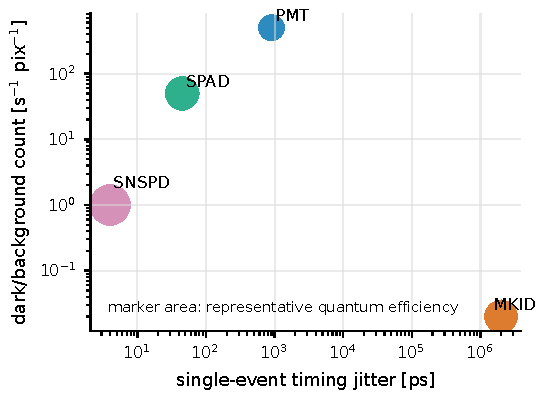
\includegraphics[width=0.72\linewidth]{figures/generated/chapter_06/ch06_detector_trade_space.pdf}
\caption{Typical operating regions of several classes of single-photon detection technology. The horizontal axis is the single-event timing jitter, the vertical axis a representative value of dark or background counts per pixel, and the point area indicates the representative quantum efficiency. PMTs suit large aperture, high flux, and ns-scale intensity interferometry; SPADs give tens-of-picoseconds timing but are limited by area and dead time; superconducting devices are strongest in low dark counts and picosecond timing but need a cryogenic system; energy-resolving detectors sacrifice timing resolution to gain the wavelength information of each photon.}
\label{fig:e13-detector-trade-space}
\end{figure}

One sentence to close this section: $\eta$ determines \emph{how many} photons become events, and thereby the "signal" in the signal-to-noise ratio; while the temporal properties of "when the event arrives and how soon the detector can fire again" determine whether the correlation structure in the event table is still faithful to the incident light field, which is exactly what the next three sections take apart.

\section{Timing jitter: why the correlation peak gets broadened}
\label{sec:e13-jitter}

Chapter~\ref{chap:e08} already foreshadowed: the detector's finite temporal response convolutionally broadens the narrow correlation peak and dilutes its height. Now we explain this thoroughly. The root of the problem is \textbf{timing jitter}: even if the same photon arrives at the same moment, the moment at which the detector output pulse is judged to be an "event" differs slightly each time, and is a random quantity. It is about tens of picoseconds for a SPAD, and can reach the ns-scale for a PMT plus electronic chain. Writing this random delay as a response function $h(t)$ (a normalized probability distribution describing "the distribution of recorded moments corresponding to the true arrival moment 0"), the observed event time is then the convolution of the true time with $h$.

For second-order correlation, each channel has its own response $h_1(t)$, $h_2(t)$, and the observed correlation excess is the convolution of the true celestial correlation with the combined response:
\begin{equation}
  C^{\rm obs}_{12}(\tau)
  =
  \int C^{\rm sky}_{12}(\tau')\,
  h_{12}(\tau-\tau')\,d\tau',
  \qquad
  h_{12}=h_1*h_2.
  \label{eq:e13-response-convolution}
\end{equation}
\begin{formulaexplain}
$C^{\rm sky}_{12}$ is the true celestial correlation, $C^{\rm obs}_{12}$ is the observed result; $h_1,h_2$ are the two channels' temporal responses, and $h_{12}$ is their convolution. The instrument "smears out" the narrow correlation peak.
\end{formulaexplain}
Here $C_{12}=g^{(2)}_{12}-1$ (dimensionless), $\tau,\tau'$ are in seconds, and $*$ is convolution. The physical picture is very plain: an infinitely narrow true correlation peak is of no use, because you simply do not know the \emph{exact} arrival moment of each photon, only that it falls within a fuzzy window of width about $\sigma$; the two fuzzy responses superpose, and the observed peak is broadened to the width of $h_{12}$.

To compute "how much broadening" precisely, use a very handy approximation: treat each response as a Gaussian. Here we single out a standard result: \emph{the convolution of two Gaussian functions is still a Gaussian, and the variances add}. Let $h_1$ be a Gaussian of width (variance) $\sigma_1^2$ and $h_2$ be a Gaussian of $\sigma_2^2$; then
\[
  h_{12}=h_1*h_2 \;\Longrightarrow\; \sigma_{12}^2=\sigma_1^2+\sigma_2^2 .
\]
Counting in the source's own width, the optical-path broadening, and the clock residual, if the terms are mutually independent the variances simply add (this is called "adding in quadrature," the general rule for the superposition of independent Gaussian broadenings):
\begin{equation}
  \sigma_{\rm obs}^2
  \simeq
  \sigma_{\rm sky}^2+\sigma_1^2+\sigma_2^2+\sigma_{\rm opt}^2+\sigma_{\rm clk}^2 .
  \label{eq:e13-jitter-budget}
\end{equation}
\begin{formulaexplain}
$\sigma_{\rm obs}$ is the observed peak width; $\sigma_{\rm sky}$ is the source's own width, $\sigma_1,\sigma_2$ are the two detectors' jitters, $\sigma_{\rm opt}$ is the optical-path broadening, and $\sigma_{\rm clk}$ is the clock residual. Independent Gaussian broadenings add in quadrature.
\end{formulaexplain}
Each term is an rms time width (seconds). $\sigma_{\rm sky}$ is the source's coherence time or pulse width, $\sigma_1,\sigma_2$ are the jitters of the detectors and electronic channels, $\sigma_{\rm opt}$ is the mirror isochronicity error (for example, the path-length differences among the different facets of a Davies--Cotton mirror), and $\sigma_{\rm clk}$ is the residual after aligning the clocks of the two stations. Here there is an important "order-of-magnitude landing": the coherence time $\tau_c$ of broadband visible light is as short as picoseconds (Chapter~\ref{chap:e02}), three orders of magnitude smaller than the ns-scale $\sigma_1,\sigma_2$, so in Eq.~\eqref{eq:e13-jitter-budget} the $\sigma_{\rm sky}$ term can almost be neglected: \emph{the observed peak width is almost entirely determined by the instrument}. VERITAS's mirror plus PMT pulse width make the intensity correlation peak describable by a Gaussian of $\sigma_\tau\simeq4\,{\rm ns}$, and the correlation peak of MAGIC-SII has a Gaussian width of about $2.2\,{\rm ns}$ \citep{2020NatAs...4.1164A,2024MNRAS.529.4387A}.

This brings a key consequence: \emph{when the peak width changes, the peak height changes too}. Because the "area" under the correlation peak (the total strength of the true correlation) is approximately conserved in the convolution, spreading it over a wider peak dilutes the peak height by the broadening factor. If the true peak width $\sigma_{\rm sky}\ll\sigma_{\rm obs}$, the observed peak height is lowered relative to the true peak height by roughly a factor of $\sigma_{\rm sky}/\sigma_{\rm obs}$. This is the quantitative source of what Chapter~\ref{chap:e08} called "the correlation peak being diluted by the temporal response," and it also explains why intensity interferometry strives so hard for high electronic bandwidth and a stable response function: the narrower the response, the less the peak-height dilution, and the easier it is to pick a peak of order $10^{-6}$ out of the noise.

\begin{figure}[tbp]
\centering
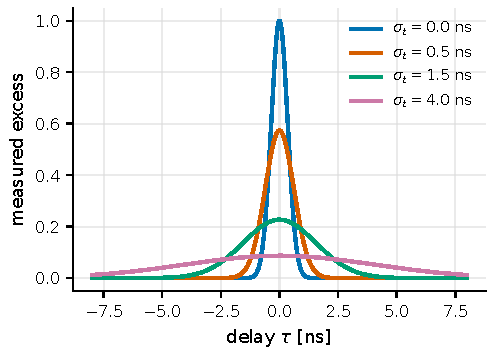
\includegraphics[width=0.72\linewidth]{figures/generated/chapter_06/ch06_detector_timing_response.pdf}
\caption{A finite temporal response broadens the narrow correlation peak and lowers its height. The curves keep the peak area approximately unchanged, changing only the rms jitter $\sigma_t$. When the true coherence time is far shorter than the ns-scale electronic response, the peak width is mainly determined by the instrument, and the peak height is diluted by the broadening factor; this is precisely why intensity interferometry needs high electronic bandwidth and a stable response function.}
\label{fig:e13-detector-timing-response}
\end{figure}

\section{Dead time and pile-up: why the recording rate saturates}
\label{sec:e13-deadtime}

Jitter changes the \emph{moment} of each event; dead time changes \emph{how many} events can be recorded. The \textbf{dead time} $\tau_d$ is a stretch of time after the detector fires during which it "catches its breath," blind to new photons. When photons come fast and dense, the dead time eats a large number of events, making the recording rate $r_{\rm rec}$ significantly lower than the true incident rate $r$: this is the count loss caused by \textbf{pile-up}. Here there is a subtle but important fork: does the dead time get "refreshed" by photons arriving during the dead time? Two answers give two models, and they must be told apart.

\paragraph{Non-paralyzable: the dead time is not refreshed}

First look at the \textbf{non-paralyzable} type. It assumes: after recording an event, the detector is dead for $\tau_d$; photons arriving during this time are all discarded, \emph{but the dead time is not extended}; once $\tau_d$ elapses, the detector immediately revives to await the next one. The derivation uses a "live-time ledger" method, done with no skipped steps.

Let the total observation duration be $T$, the true incident rate be $r$ (${\rm s}^{-1}$), and the total number of recorded events be $M$. Each recorded event brings $\tau_d$ of dead time, so the total dead time is $M\tau_d$, and hence the time the detector is truly "alive and responsive" is
\[
  T_{\rm live}=T-M\tau_d .
\]
The key to the non-paralyzable type is: only photons arriving during the live time are recorded, and during the live time photons arrive Poissonianly at the true rate $r$, so
\[
  M=r\,T_{\rm live}=r\,(T-M\tau_d).
\]
Gathering the terms containing $M$:
\[
  M=rT-rM\tau_d \;\Longrightarrow\; M+rM\tau_d=rT \;\Longrightarrow\; M(1+r\tau_d)=rT .
\]
Divide both sides by $T$ and write $r_{\rm rec}=M/T$ to obtain the recording rate:
\begin{equation}
  r_{\rm rec}=\frac{r}{1+r\tau_d}.
  \label{eq:e13-nonparalyzable}
\end{equation}
\begin{formulaexplain}
$r$ is the true incident rate, $r_{\rm rec}$ is the recording rate, and $\tau_d$ is the dead time. In the non-paralyzable type, photons within the dead time are discarded but do not extend the recovery window, so $r_{\rm rec}$ rises monotonically with $r$ and saturates to $1/\tau_d$.
\end{formulaexplain}
Read the limits of this formula. At low flux $r\tau_d\ll1$, the denominator approaches 1, $r_{\rm rec}\approx r(1-r\tau_d)$, and the loss is small; at high flux $r\tau_d\gg1$, $r_{\rm rec}\to 1/\tau_d$: the recording rate \emph{saturates} at an upper limit, the detector reporting at most one event every $\tau_d$, no matter how many more photons crowd in, but it never retreats.

\paragraph{Paralyzable: every photon refreshes the dead time}

Now look at the \textbf{paralyzable} type. It assumes: every new photon arriving during the dead time, though \emph{not recorded}, \emph{re-triggers} a fresh stretch of $\tau_d$ dead time. So a photon is recorded only when, at the moment it arrives, it has been \emph{empty for at least $\tau_d$} with no photons before it.

The derivation uses a standard result of the Poisson process: for a Poisson process of rate $r$, the time interval between two adjacent photons follows an exponential distribution, and \emph{the probability that the interval exceeds $\tau_d$ is $e^{-r\tau_d}$}. (This is the probability that "there is not a single photon in a window of length $\tau_d$," equal to the Poisson distribution taking 0: $P(0)=e^{-r\tau_d}$.) An arriving photon can be recorded if and only if the gap before it is greater than $\tau_d$. All photons arrive at rate $r$, and only the fraction whose "preceding gap $>\tau_d$" counts, so the recording rate is
\[
  r_{\rm rec}=r\times P(\text{preceding interval}>\tau_d)=r\,e^{-r\tau_d}.
\]
Written as a numbered formula:
\begin{equation}
  r_{\rm rec}=r\,e^{-r\tau_d}.
  \label{eq:e13-paralyzable}
\end{equation}
\begin{formulaexplain}
Likewise a dead-time model, but every arriving photon refreshes the recovery window. Hence $r_{\rm rec}$ reaches its maximum at $r\tau_d=1$, and thereafter \emph{decreases} as $r$ increases: at high flux the detector is almost continuously refreshed and reports no events.
\end{formulaexplain}
Read the limits: at low flux $r\tau_d\ll1$, $e^{-r\tau_d}\approx1-r\tau_d$, $r_{\rm rec}\approx r(1-r\tau_d)$, \emph{completely identical} to the non-paralyzable type at low flux, which is why the two models are hard to distinguish in weak light. But high flux is entirely different: differentiating $r_{\rm rec}=re^{-r\tau_d}$ with respect to $r$, $\frac{d r_{\rm rec}}{dr}=e^{-r\tau_d}(1-r\tau_d)$, which is zero at $r\tau_d=1$ (i.e. $r=1/\tau_d$), a maximum, with peak value $r_{\rm rec}^{\max}=1/(e\tau_d)\approx0.368/\tau_d$; beyond this, the photons are so dense that they continuously refresh the dead time, and the recording rate \emph{turns downward}, in the extreme leaving the detector almost paralyzed (hence the name of the model).

\paragraph{Comparison and orders of magnitude}

Reading the two formulas side by side, the physical difference in one sentence: the non-paralyzable type \emph{saturates} to $1/\tau_d$ at high flux, while the paralyzable type \emph{falls back} at high flux. This difference is critical experimentally: if you mistake a paralyzable type for a non-paralyzable one, you will severely overestimate the true rate at high count rates. So a real instrument must \emph{separately measure} which class it belongs to and what $\tau_d$ is, the method being to plot the curve of $r_{\rm rec}$ versus $r$ using a stable light source of adjustable intensity, and see whether it saturates or falls back.

Plug in numbers to get a feel for the magnitude. Take a typical dead time of a high-speed single-photon channel, $\tau_d=20\,{\rm ns}=2\times10^{-8}\,{\rm s}$:
\[
  r=10^7\,{\rm s^{-1}}:\quad r\tau_d=0.2,\quad
  r_{\rm rec}^{\rm non}=\frac{10^7}{1.2}\approx8.3\times10^6\,{\rm s^{-1}},
\]
that is, already a loss of about $17\%$; at the same incident rate the paralyzable type gives $r_{\rm rec}=10^7e^{-0.2}\approx8.2\times10^6\,{\rm s^{-1}}$, almost identical. Raising further to $r=10^8\,{\rm s^{-1}}$ ($r\tau_d=2$): the non-paralyzable type gives $r_{\rm rec}=10^8/3\approx3.3\times10^7\,{\rm s^{-1}}$, still climbing; the paralyzable type gives $r_{\rm rec}=10^8e^{-2}\approx1.35\times10^7\,{\rm s^{-1}}$, \emph{already over the peak and falling} (the peak occurs at $r=1/\tau_d=5\times10^7\,{\rm s^{-1}}$, where $r_{\rm rec}^{\max}\approx1.84\times10^7\,{\rm s^{-1}}$). SPADs commonly have dead times of tens of ns to a few hundred ns, energy-resolving detectors can reach the $100\,\mu{\rm s}$ scale, and modern TCSPC electronics can compress the channel dead time to 650 ps, though the detector pulse width and front-end electronics still limit the real high-flux capability \citep{2009A&A...508..531N,2013PASP..125.1348M,2020RScI...91a3108W}.

\begin{figure}[tbp]
\centering
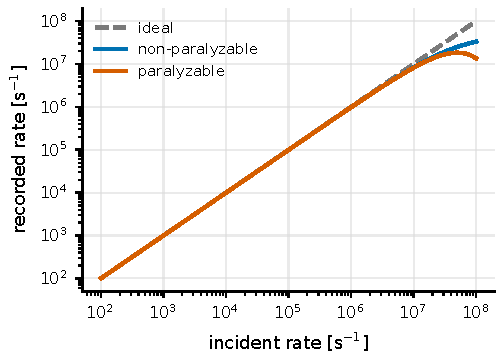
\includegraphics[width=0.72\linewidth]{figures/generated/chapter_06/ch06_deadtime_saturation.pdf}
\caption{As the incident count rate rises, dead time makes the recorded count rate deviate from the ideal straight line. The non-paralyzable type tends to the saturation value $1/\tau_d$, while the paralyzable type instead decreases at extremely high flux. The figure takes $\tau_d=20\,{\rm ns}$, representing the order of magnitude of a high-speed single-photon channel; a real instrument needs to measure $\tau_d$ and the model type separately using an adjustable-intensity light source.}
\label{fig:e13-deadtime-saturation}
\end{figure}

Dead time also hints at a trick commonly used in intensity interferometry: \textbf{split the light onto two independent detectors} for cross-correlation (the HBT approach, see Chapter~\ref{chap:e10}). Because the dead time is \emph{each detector's own}, the two detectors will not both miss a coincidence near zero delay because the other is in its dead time; this both raises the total count rate that can be tolerated and, as a bonus, suppresses the same-channel afterpulsing discussed in the next section \citep{1957RSPSA.242..300B,1996ApOpt..35.1956C,2020RScI...91a3108W}.

\section{Afterpulsing: short-delay false correlations the detector makes itself}
\label{sec:e13-afterpulse}

Dead time makes events \emph{fewer}, but afterpulsing makes events \emph{appear out of nothing}. In avalanche-type devices (SPAD, SiPM), an avalanche has some carriers "captured" by material defects (traps), which are released a while later and re-trigger a secondary pulse having nothing to do with celestial photons: this is the \textbf{afterpulse}. Its danger lies in this: these false pulses always follow closely behind the true pulse by a few ns to a few $\mu$s, falling exactly in the \emph{short-delay} interval we care about most, and forge a false peak in the autocorrelation, misread as "photons arriving in company."

Write it in rate form. Let the probability that each true event produces an afterpulse be $\epsilon_{\rm ap}$, and the delay of these afterpulses relative to the main pulse follow a normalized distribution $k_{\rm ap}(\tau)$; then the extra event rate is
\begin{equation}
  R_{\rm ap}(\tau)=\epsilon_{\rm ap}\,R_{\rm det}\,k_{\rm ap}(\tau),
  \qquad
  \int_0^\infty k_{\rm ap}(\tau)\,d\tau=1.
  \label{eq:e13-afterpulse}
\end{equation}
\begin{formulaexplain}
$R_{\rm ap}$ is the afterpulse contribution; $\epsilon_{\rm ap}$ is the probability that each true event produces an afterpulse; $R_{\rm det}$ is the true detection rate; $k_{\rm ap}$ is the normalized delay kernel. It describes the short-delay false correlation the detector \emph{makes itself}.
\end{formulaexplain}
Let us pin down each term. $\epsilon_{\rm ap}$ is dimensionless, ranging from $10^{-4}$ to $10^{-2}$ depending on the device and gating scheme; $R_{\rm det}$ is the detection rate given by Eq.~\eqref{eq:e13-detected-rate} (${\rm s}^{-1}$); $k_{\rm ap}(\tau)$ is in units of ${\rm s}^{-1}$ (because it integrates to unity over $\tau$), and its characteristic time ranges from ns to $\mu$s. The structure of the formula is "true event rate $\times$ single-afterpulse probability $\times$ delay distribution," very easy to remember.

How to distinguish it from a true signal? Two methods. First, do the autocorrelation \emph{on the same detector}, and you will see the afterpulse peak conspicuously appear at short delays; second, do the cross-correlation \emph{on two independent detectors}, and because the trap releases of detectors A and B are mutually independent and not synchronized, the afterpulses do not create coincidences in the cross-correlation and are thus greatly suppressed. This once again shows the double benefit of HBT beam-split cross-correlation: it both solves dead time and evades afterpulsing: the same light, split to two "mutually oblivious" detectors, so neither can use its own defects to contaminate the other's coincidence counts \citep{1957RSPSA.242..300B,1996ApOpt..35.1956C,2020RScI...91a3108W}.

\section{Clocks and synchronization: putting two telescopes on the same time axis}
\label{sec:e13-clock}

By now, the event table inside a single telescope has been built. But intensity interferometry and very-long-baseline timing need at least \emph{two} telescopes, and their respective event tables can only be correlated once placed on a \emph{common time axis}. This requires the clocks of the two stations to be aligned accurately enough. How accurate is enough? Here is a conversion that runs through the whole book, translating "timing precision" into "the distance light travels":
\begin{equation}
  \Delta\ell = c\,\Delta t .
  \label{eq:e13-lightpath}
\end{equation}
\begin{formulaexplain}
$\Delta t$ is the residual of aligning the two stations' clocks, $c$ is the speed of light, and $\Delta\ell$ is the distance light travels in this time. It directly converts "synchronized to how many picoseconds" into "equivalent to how many centimetres of path length."
\end{formulaexplain}
This formula is in fact the "time--path-length" correspondence used in Chapter~\ref{chap:e01}, only this time applied to clocks. Plug in numbers (CGS, $c=3\times10^{10}\,{\rm cm\,s^{-1}}$): $\Delta t=1\,{\rm ns}=10^{-9}\,{\rm s}$ corresponds to $\Delta\ell=30\,{\rm cm}$; $\Delta t=100\,{\rm ps}$ corresponds to $3\,{\rm cm}$; $\Delta t=1\,{\rm ps}$ corresponds to $0.3\,{\rm mm}$. So "synchronizing the two stations to the picosecond-nanosecond" is physically equivalent to "aligning the lengths of the two optical paths to the millimetre-centimetre", a very intuitive scale. Conversely, as long as you align the clocks to a few tens of picoseconds, a path-length difference within a few centimetres is absorbed by the clock.

There are two mainstream routes to achieving this synchronization. One is \textbf{GPS timing}: the satellite-broadcast pulse-per-second (PPS) gives each station a common absolute moment, complemented by a local rubidium clock for short-term stability; AquEYE/Iqueye use a rubidium clock plus GPS PPS to achieve a \emph{relative} time precision of about 100 ps rms and keep the \emph{absolute} UTC precision within $0.5\,{\rm ns}$ \citep{2009A&A...508..531N,2015SPIE.9504E..0CZ}. The other is \textbf{White Rabbit}: an Ethernet-based fibre synchronization protocol with precise phase measurement, which distributes one master clock via fibre to each station and compensates for the fibre length in real time; a 5 km fibre link test obtained a synchronization contribution of about 39 ps, which, converted by Eq.~\eqref{eq:e13-lightpath}, is equivalent to only about 1.2 cm of path-length residual \citep{2013NIMPA.725..187J,2020RScI...91a3108W}.

With a common clock, one must still subtract a larger, \emph{time-varying} term: the geometric delay. The same starlight arrives at the two stations at different moments, because the path lengths from the two stations to the source are unequal. For a pair of stations $a,b$:
\begin{equation}
  \Delta t_{\rm geo}(t)
  =
  \frac{\mathbf{B}_{ab}(t)\cdot\hat{\mathbf{s}}}{c},
  \qquad
  \mathbf{B}_{ab}=\mathbf{r}_b-\mathbf{r}_a .
  \label{eq:e13-geometric-delay}
\end{equation}
\begin{formulaexplain}
$\Delta t_{\rm geo}$ is the geometric delay between the two stations; $\mathbf B_{ab}$ is the baseline vector (given by the difference of the two stations' positions), $\hat{\mathbf s}$ is the unit vector of the source direction, and $c$ is the speed of light. It \emph{projects} the spatial baseline into the amount of time by which the two event tables must be shifted relative to each other.
\end{formulaexplain}
$\mathbf B_{ab}$ is in units of m, $\hat{\mathbf s}$ is dimensionless, the dot product $\mathbf B_{ab}\cdot\hat{\mathbf s}$ is the projected length of the baseline onto the source direction, and dividing by $c$ gives the time. Plug in numbers: a 100 m baseline gives at most $\Delta t_{\rm geo}=100/(3\times10^8)\approx333\,{\rm ns}$ (this maximum occurs when the source direction is parallel to the baseline, i.e. near the horizon; conversely, when the source is at the zenith and the baseline is nearly horizontal, the projection $\mathbf B_{ab}\cdot\hat{\mathbf s}\approx0$ and the geometric delay is near zero), and a 1 km baseline about $3.3\,\mu{\rm s}$, far larger than the picosecond-scale detector jitter, showing that the geometric delay is the \emph{largest} time term in the correlation, and must be subtracted first before aligning zero delay. More troublesome, it \emph{drifts with time}: Earth's rotation continuously changes the projected baseline, and a 100 m baseline drifts fastest near the zenith (culmination), with a delay change rate of about $\Omega_\oplus B/c\sim2.4\times10^{-11}\,{\rm s\,s^{-1}}$, where $\Omega_\oplus\approx7.3\times10^{-5}\,{\rm rad\,s^{-1}}$ is Earth's rotation angular velocity; this means about $24\,{\rm ps}$ of drift per second (about $25\,{\rm ns}$ accumulated over 17 minutes); for a picosecond-scale peak shape, this cannot be absorbed once and for all by a constant delay. VERITAS-SII applies a shifting time-lag correction for the geometric path per correlation frame, and MAGIC-SII applies a variable time-delay correction after the Pearson correlation \citep{2020NatAs...4.1164A,2024MNRAS.529.4387A}.

If one also wants to fold photons into a pulsar phase, or compare arrival times with other bands, the station time must be further converted to the \emph{Solar System barycenter} (SSB), adding a string of standard correction terms: the conversion from the local clock to coordinate time, the Roemer light-travel time (Earth's orbit around the Sun gives at most about $\pm500\,{\rm s}$), the Einstein gravitational/motional clock-rate correction, the Shapiro gravitational delay, and the atmospheric delay. Tempo2 has done these corrections to the ns level, and barycorrpy and Astropy provide Python-workflow interfaces \citep{2006MNRAS.369..655H,2006MNRAS.372.1549E,2018RNAAS...2....4K,2013A&A...558A..33A,2018AJ....156..123A}. These belong to the advanced content of absolute timing; for this chapter one need only remember: same-night intensity correlation looks at \emph{relative} delays, and only pulse phase and multi-messenger comparison need \emph{absolute} barycentric time.

\begin{figure}[tbp]
\centering
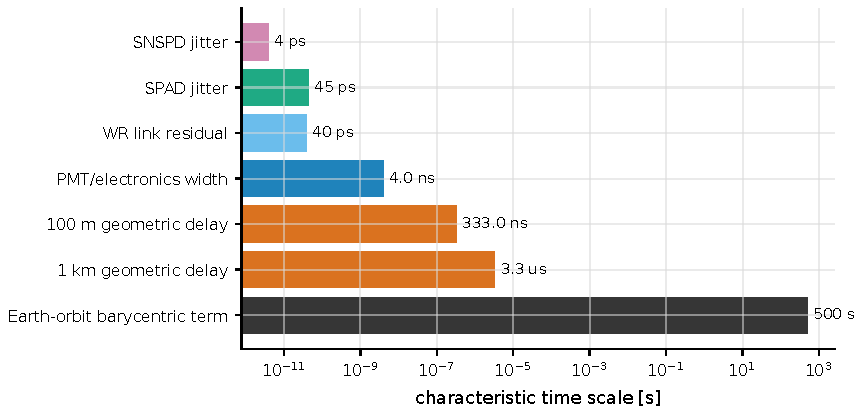
\includegraphics[width=0.84\linewidth]{figures/generated/chapter_06/ch06_time_budget.pdf}
\caption{The same event table simultaneously encounters time terms of picosecond, nanosecond, microsecond, and hundred-second scale. Detector jitter and the White Rabbit residual determine whether the correlation peak can keep its narrow shape; electronic and mirror responses determine the ns-scale intensity-interferometry peak width; the geometric delay is determined by the baseline length and source direction, and drifts with Earth's rotation; the Solar-System barycentric correction, though not a same-night peak-width term, is the absolute time basis for pulse phase, cross-night combination, and multi-messenger comparison.}
\label{fig:e13-time-budget}
\end{figure}

Writing all these delays into the calibrated event table, the raw counter time becomes a physical time comparable across stations:
\begin{equation}
  t^{\rm cal}_q =
  t^{\rm raw}_q
  +\Delta_{\rm clk}(t_q)
  +\Delta_{\rm elec}(a_q,d_q)
  +\Delta_{\rm det}(\lambda_q,d_q)
  -\frac{\mathbf{r}_{a_q}(t_q)\cdot\hat{\mathbf{s}}}{c}.
  \label{eq:e13-calibrated-time}
\end{equation}
\begin{formulaexplain}
$t_q^{\rm cal}$ is the corrected event time; $\Delta_{\rm clk},\Delta_{\rm elec},\Delta_{\rm det}$ respectively correct for the clock, electronic-link, and detector delays; the last term subtracts the geometric light-travel time. It places different stations on a common time axis.
\end{formulaexplain}
$\Delta_{\rm clk}$ is the offset of the local clock relative to the unified time scale (tens of picoseconds to ns), $\Delta_{\rm elec}$ is the fixed or slowly drifting delay of cables, amplifiers, discriminators, and ADC/TDC channels (commonly calibrated with a pulse source and loopback links), $\Delta_{\rm det}$ is the internal detector delay (which may depend on wavelength, bias, temperature, and pulse height), and the last term is exactly the geometric delay of Eq.~\eqref{eq:e13-geometric-delay}. This formula gathers all the delay terms of the previous sections into a unified time-calibration framework.

\section{The event-table fields: why every column must be kept}
\label{sec:e13-schema}

Now we can answer the most practical question from the start of the chapter: which fields should the event table store, exactly? The answer is to store in \emph{three layers}, and the raw layer must never be overwritten by post-processing.

The \textbf{raw layer} stores the quantities from Eq.~\eqref{eq:e13-raw-event} that are "closest to the electronics": the counter tick $n_q$, the telescope/station number $a_q$, the detector number $d_q$, the wavelength channel $c_q$, the polarization channel $p_q$, the quality flag $f_q$, and the weight $w_q$. Why can no column be omitted? Because each corresponds to a kind of \emph{choice you might still want to redo afterwards}: keeping $n_q$ lets you re-bin and re-do the delay correction; keeping $a_q,d_q$ lets you do \emph{cross}-correlation rather than autocorrelation (thereby evading dead time and afterpulsing); keeping $c_q$ lets you re-select frequency by wavelength afterwards; keeping $p_q$ lets you reconstruct polarization (polarization reconstruction is deferred to a later chapter, see Chapter~\ref{chap:e22}); keeping $f_q$ lets you trace the origin of an anomalous peak; keeping $w_q$ lets you do weighted analysis. Once this layer is compressed into a light curve, all these "redoings" become impossible.

The \textbf{calibrated layer} turns the raw ticks, via Eq.~\eqref{eq:e13-calibrated-time}, into physical time on a unified time axis, and adds physical quantities such as telescope attitude, wavelength, polarization, and weight. It is the product of "each analysis version," which can be updated as the calibration improves, but each time one must record which set of corrections was used. The \textbf{correlation-product layer} finally records the baseline, delay grid, bin width, correlation amplitude, rejection conditions, and covariance, that is, the "finished products" such as $g^{(2)}(\tau)$, $|V|^2$, or pulse arrival times.

How large is the data volume? It is determined by the event rate and the bytes per event:
\begin{equation}
  \dot{M}
  \simeq
  N_{\rm tel}\,N_{\rm ch}\,R_{\rm evt}\,N_{\rm byte}.
  \label{eq:e13-data-rate}
\end{equation}
\begin{formulaexplain}
$\dot M$ is the data rate; $N_{\rm tel}$ is the number of telescopes, $N_{\rm ch}$ the number of channels per telescope, $R_{\rm evt}$ the single-channel event rate, and $N_{\rm byte}$ the bytes per event. It estimates the storage pressure of an event table or waveform stream.
\end{formulaexplain}
$\dot M$ is in units of ${\rm byte\,s^{-1}}$. Plug in numbers: $N_{\rm tel}=4$, $N_{\rm ch}=8$, $R_{\rm evt}=10^6\,{\rm s^{-1}}$, $N_{\rm byte}=16$, then $\dot M\simeq4\times8\times10^6\times16=5.12\times10^8\,{\rm byte\,s^{-1}}\approx512\,{\rm MB\,s^{-1}}$. Continuous waveform sampling is even fiercer: VERITAS-SII continuously digitizes each telescope's PMT signal at 250 MS/s, about 250 MB/s per telescope, with the total data volume of an entire experiment reaching tens of TB \citep{2020NatAs...4.1164A}. As for storage format, the FITS BINTABLE extension suits long-term archiving and astronomical-software interoperability, while HDF5/Parquet suit high-throughput columnar filtering; Astropy provides interfaces for FITS, coordinate, and time processing, making it convenient to put the event table, time-scale conversion, and barycentric correction into the same Python analysis chain \citep{2010A&A...524A..42P,2013A&A...558A..33A,2018AJ....156..123A}.

The meaning of layering, in one sentence: it lets later readers regenerate light curves, $g^{(2)}(\tau)$, spatial visibilities, or pulse arrival times \emph{from the same raw data}, without having to guess which choices early scripts quietly made. Reproducibility is the highest principle of event-table design.

\section{The trade-off between spectral resolution and coherence time}
\label{sec:e13-spectral}

One last field deserves separate treatment: the wavelength channel $c_q$. Tagging each photon with a wavelength is not just for spectroscopy, but even more because \emph{the width of the wavelength channel directly determines the coherence time}, and the coherence time in turn determines the intrinsic width of the correlation peak. Recall Chapters~\ref{chap:e02} and~\ref{chap:e08}: the narrower the channel, the longer the phase memory of the electric field. Quantitatively, if the channel is approximately rectangular with central wavelength $\lambda$ and width $\Delta\lambda$:
\begin{equation}
  \tau_c
  \simeq
  \frac{1}{\Delta\nu}
  \simeq
  \frac{\lambda^2}{c\,\Delta\lambda}
  =
  \frac{R\,\lambda}{c},
  \qquad
  R=\frac{\lambda}{\Delta\lambda}.
  \label{eq:e13-coherence-time}
\end{equation}
\begin{formulaexplain}
$\tau_c$ is the coherence time; $\Delta\nu$ is the frequency bandwidth; $\lambda,\Delta\lambda$ are the central wavelength and wavelength bandwidth; $R=\lambda/\Delta\lambda$ is the spectral resolution. A narrow channel lengthens the phase memory, but lowers the single-channel photon rate.
\end{formulaexplain}
Do not skip the two middle steps. The first step $\tau_c\simeq1/\Delta\nu$ is the bandwidth--coherence-time relation of Chapter~\ref{chap:e02}. The second step converts $\Delta\nu$ into a wavelength quantity: differentiating $\nu=c/\lambda$, $|d\nu|=(c/\lambda^2)\,|d\lambda|$, so $\Delta\nu\simeq c\Delta\lambda/\lambda^2$, giving $\tau_c\simeq\lambda^2/(c\Delta\lambda)$. The third step recognizes $R=\lambda/\Delta\lambda$, so $\lambda^2/(c\Delta\lambda)=(\lambda/\Delta\lambda)(\lambda/c)=R\lambda/c$. All three steps are identity transformations, with no extra approximation.

Plug in numbers ($\lambda=500\,{\rm nm}$): $R=100\Rightarrow\tau_c\simeq100\times500\times10^{-9}/(3\times10^8)\approx0.17\,{\rm ps}$; $R=10^4\Rightarrow\tau_c\simeq17\,{\rm ps}$; $R=10^5\Rightarrow\tau_c\simeq170\,{\rm ps}$. Note: even at $R=10^5$, $\tau_c$ is still shorter than the ns response of most PMTs/electronic chains, so by the conclusion of Section~\ref{sec:e13-jitter}, the actual correlation peak width is \emph{still determined by the instrument}; raising $R$ lengthens the phase memory (thereby affecting the ratio of electronic to optical bandwidth in the peak \emph{height}), rather than making the peak narrower.

Hence the final trade-off of the chapter. Raising $R$ (using a narrower filter) lengthens $\tau_c$ and makes the coherence "purer," but at the same time lowers the single-channel photon rate by about $1/R$ (the narrower the bandwidth, the fewer photons come in). To have both, one must \emph{read out more wavelength channels simultaneously} to make up the total flux: multi-channel TCSPC can treat different wavelengths as independent inputs and output a single time-ordered data stream; whereas the SII systems of MAGIC and VERITAS go the other way, choosing a few wide filter channels to gain a higher photon rate: VERITAS uses a filter centred at 416 nm with an effective width of 13 nm, and MAGIC uses an interference filter of 425 nm and 26 nm \citep{2020NatAs...4.1164A,2024MNRAS.529.4387A,1974iiia.book.....H}. Choosing wide or narrow depends on the science goal: to measure a stellar diameter, a wide channel that boosts the signal-to-noise ratio is fine; but to study emission lines, absorption lines, or the velocity structure of a rapid rotator, wavelength-resolved correlation can directly give "how the spatial information varies with velocity," and then the price of a narrow channel is worth paying.

\begin{figure}[tbp]
\centering
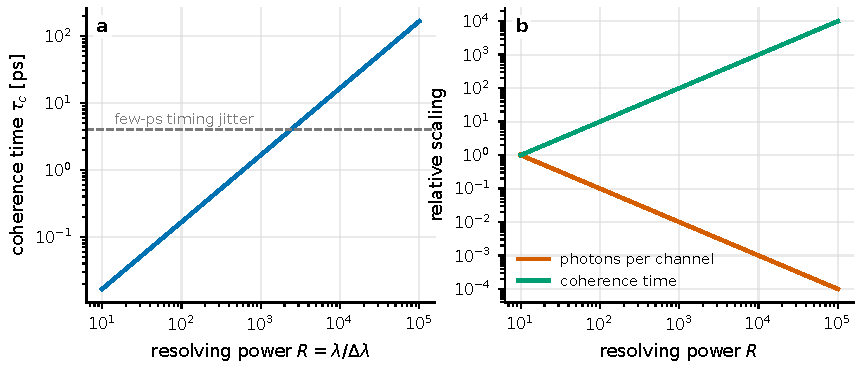
\includegraphics[width=0.92\linewidth]{figures/generated/chapter_06/ch06_spectral_resolution_coherence.pdf}
\caption{The order-of-magnitude relation between spectral resolution and coherence time. The left panel fixes $\lambda=500\,{\rm nm}$ and shows $\tau_c\simeq R\lambda/c$ growing linearly with resolution; the right panel shows the single-channel photon rate falling roughly as $1/R$ while the coherence time increases with $R$. The dependence of ideal intensity-interferometry signal-to-noise on optical bandwidth partly cancels, but a real instrument is further limited by filter shape, detector response, background, and electronic bandwidth.}
\label{fig:e13-spectral-resolution-coherence}
\end{figure}

\section{Chapter Summary}
\label{sec:e13-summary}

\begin{itemize}
  \item \textbf{A photon must pass several checkpoints to become an event.} The quantum efficiency $\eta$ determines "how many photons become events" (Eq.~\eqref{eq:e13-detected-rate}); PMTs offer large area and high gain, SPADs/SiPMs offer single-photon picosecond timing but are limited by area, dead time, and afterpulsing; each has its trade-offs.
  \item \textbf{Jitter broadens the correlation peak and dilutes its height.} The observed peak is the convolution of the true peak with the instrument response (Eq.~\eqref{eq:e13-response-convolution}); independent Gaussian broadenings add in quadrature, $\sigma_{\rm obs}^2=\sum\sigma_i^2$ (Eq.~\eqref{eq:e13-jitter-budget}). Visible-light $\tau_c\sim$ps is far smaller than the ns-scale response, so the peak width is almost entirely determined by the instrument, and the peak height is diluted by $\sim\sigma_{\rm sky}/\sigma_{\rm obs}$, echoing Chapter~\ref{chap:e08}.
  \item \textbf{Dead time saturates the recording rate, and comes in two types.} The non-paralyzable type $r_{\rm rec}=r/(1+r\tau_d)$ (Eq.~\eqref{eq:e13-nonparalyzable}) saturates at high flux to $1/\tau_d$; the paralyzable type $r_{\rm rec}=re^{-r\tau_d}$ (Eq.~\eqref{eq:e13-paralyzable}) peaks at $r\tau_d=1$ and then falls back. They coincide at weak light but differ vastly at strong light, so the type must be measured.
  \item \textbf{Afterpulsing forges false short-delay peaks.} The afterpulse rate $R_{\rm ap}=\epsilon_{\rm ap}R_{\rm det}k_{\rm ap}(\tau)$ (Eq.~\eqref{eq:e13-afterpulse}) falls in the crucial short-delay region. Splitting to two independent detectors for cross-correlation resolves dead time and afterpulsing at once.
  \item \textbf{Clock synchronization is equivalent to aligning path lengths.} $\Delta\ell=c\Delta t$ (Eq.~\eqref{eq:e13-lightpath}): 100 ps $\leftrightarrow$ 3 cm, 1 ns $\leftrightarrow$ 30 cm. GPS/White Rabbit align the two stations to tens of picoseconds; the geometric delay $\Delta t_{\rm geo}=\mathbf B\cdot\hat{\mathbf s}/c$ (Eq.~\eqref{eq:e13-geometric-delay}) is the largest (about 333 ns for a hundred-metre baseline) and drifts with Earth's rotation, and must be subtracted frame by frame.
  \item \textbf{The event table has three layers, preserving the raw information.} The raw layer cannot be overwritten, the calibrated layer can be iterated, and the correlation-product layer delivers finished products; each field corresponds to a "redoing you might still want afterwards." Reproducibility is the highest principle.
  \item \textbf{Spectral resolution and coherence time trade off against each other.} $\tau_c\simeq R\lambda/c$ (Eq.~\eqref{eq:e13-coherence-time}): the larger $R$, the longer the coherence time, but the single-channel photon rate falls by about $1/R$. Choosing wide or narrow depends on whether you are measuring a diameter or studying velocity structure.
\end{itemize}

\noindent\textbf{Questions to Ponder.} (1) If a SPAD's dead-time curve first rises and then falls at high flux, which type is it more likely to be? Based on this, how do you infer $\tau_d$ backwards? (2) Aligning two stations' clocks to 50 ps is equivalent to aligning how long a path length? Is this large or small relative to the geometric delay of a 100 m baseline? (3) If you raise $R$ from 100 to $10^4$, by how many times does the coherence time increase, and to about what fraction does the single-channel photon rate fall? What should be done to preserve the total flux?
